\section{Examples of Functions of Multiple Variables}
\label{sec:examples}

\subsection{Pre-Calculus Idea -- Topological Maps}
If you’ve ever hiked, you have probably seen a topographical map. Figure \ref{fig:4-1-topo} shows part of a topographic map of Stowe, Vermont.

\begin{figure}[!ht]
  \centering
    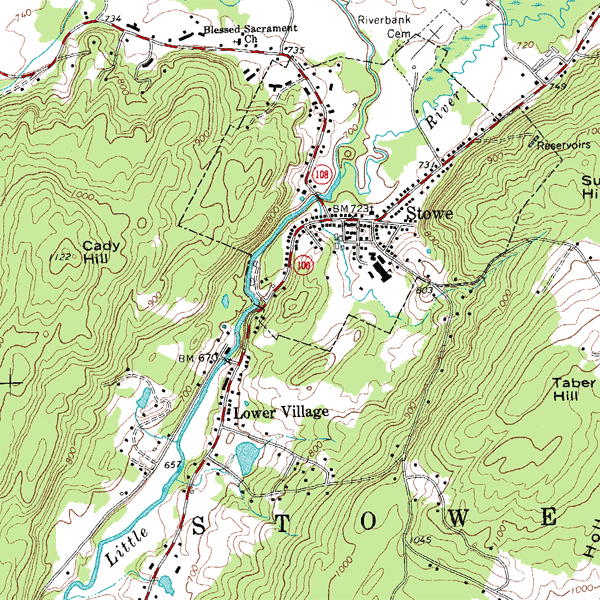
\includegraphics[width=0.4\textwidth]{img/chap4/image001.png}
    \caption{Topographical map of Stowe, VT: USGS, \url{http://en.wikipedia.org/wiki/File:Topographic_map_example.png.}}
    \label{fig:4-1-topo}
\end{figure}

Points with the same elevation are connected with curves, so you can read not only your east-west and your north-south location, but also your elevation. You may have also seen weather maps that use the same principle -- points with the same temperature are connected with curves (isotherms), or points with the same atmospheric pressure are connected with curves (isobars). These maps let you read not only a place's location but also its temperature or atmospheric pressure.

In this chapter, we will use that same idea to make graphs of functions of two variables.
